\documentclass[journal]{IEEEtran}

% Packages
\usepackage{amsmath,amssymb,amsfonts}
\usepackage{booktabs}
\usepackage{graphicx}
\usepackage{multirow}
\usepackage{array}
\usepackage{url}
\usepackage{xcolor}
\usepackage{balance}

% Custom commands (matching parent paper GE_manuscript.tex)
\newcommand{\E}{\mathcal{E}}               % Economic decision complex
\newcommand{\M}{\mathcal{M}}               % General manifold
\newcommand{\BF}{\mathrm{BF}}              % Behavioral friction
\DeclareMathOperator*{\argmin}{arg\,min}

\begin{document}

\onecolumn
\begingroup
\small
\input{response_body.tex}
\endgroup
\twocolumn

\title{Geometric Prediction of Economic Behavior:\\Cross-Domain Validation Across Game Theory\\and Prospect Theory}

\author{Andrew~H.~Bond,~\IEEEmembership{Senior Lecturer}%
\thanks{A.~H.~Bond is with the Department of Computer Engineering, San Jos\'{e} State University, San Jos\'{e}, CA 95192 USA (e-mail: andrew.bond@sjsu.edu; ORCID: 0009-0003-2599-6158).}%
\thanks{Manuscript received \today.}}

\markboth{IEEE Transactions on Computational Social Systems}%
{Bond: Geometric Prediction of Economic Behavior}

\maketitle

\begin{abstract}
We study a geometric framework for economic decision-making in which choices are represented as displacements on a 9-dimensional decision manifold and evaluated by a Mahalanobis cost metric.
A diagonal covariance matrix~$\Sigma$ is selected on nine bargaining and public-goods targets by exhaustive structural search over active dimensions and is then evaluated on seven held-out targets from prospect-theory and historical-replication settings.
On the present 16-target aggregate benchmark, the selected model activates Social Impact ($d_6$, $\sigma^2=78.26$), Virtue/Identity ($d_7$, $\sigma^2=32.28$), and Epistemic Status ($d_9$, $\sigma^2=0.013$), yielding MAE\,=\,2.70\% and 16/16 matches within stated engineering tolerances.
The monetary dimension ($d_1$) is inactive in this benchmark, a result we interpret as a context-specific diagnostic rather than a universal claim that monetary stakes never matter.
The revision makes the model self-contained, separates the covariance metric from researcher-coded encodings, reports a conservative parameter/flexibility accounting, and adds uncertainty estimates where individual-level data are recoverable.
The evidence should be read as a falsifiable cross-domain modeling result, not as a definitive unification of game theory and prospect theory.
\end{abstract}

\begin{IEEEkeywords}
Computational social systems, geometric economics, behavioral prediction, game theory, prospect theory, Mahalanobis distance, bounded rationality, manifold learning, cross-domain validation, structural fuzzing.
\end{IEEEkeywords}


%==============================================================================
\section{Introduction}
\label{sec:intro}
%==============================================================================

\IEEEPARstart{P}{redicting} economic behavior is a central problem for computational social systems because social platforms, markets, energy systems, and policy mechanisms all depend on agents whose choices are neither purely monetary nor fully random.
Expected-utility theory, axiomatized by von~Neumann and Morgenstern~\cite{vonneumann1944} and extended by Savage~\cite{savage1954}, provides a clean scalar account of choice under risk.
Behavioral economics has shown, however, that actual choices also reflect reference dependence, loss aversion, probability weighting, fairness, reciprocity, and social meaning~\cite{kahneman1979,tversky1992,fehr1999,bolton2000}.
Large replications further show that many prospect-theory patterns are robust across countries while also exhibiting meaningful heterogeneity~\cite{ruggeri2020,henrich2010}.

Existing models typically specialize by domain.
Cumulative Prospect Theory (CPT)~\cite{tversky1992} is powerful for risky lotteries but is not a model of strategic interaction.
Fehr--Schmidt inequality aversion~\cite{fehr1999} and ERC~\cite{bolton2000} address social preferences in games but do not model certainty effects, reflection effects, or probability weighting.
Computational game-theoretic models in complex socio-technical systems often represent agents through payoffs, strategies, reinforcement rules, or negotiation protocols, but they still require a behavioral primitive specifying which features of a situation are costly or attractive to the agent.

This paper investigates whether such a behavioral primitive can be represented geometrically.
We model each economic scenario as a pair of displacement vectors in a 9-dimensional decision space~$\E$.
The dimensions encode monetary consequences, rights or entitlements, fairness, autonomy, privacy/trust, social impact, virtue/identity, legitimacy, and epistemic status.
A covariance matrix~$\Sigma$ determines the cost of movement along these dimensions through Mahalanobis distance, and a softmax choice rule maps relative costs to population choice frequencies.

The empirical design is deliberately modest.
We select a diagonal covariance matrix on nine game-theoretic targets and then evaluate the same metric, without re-estimating the variances, on seven held-out targets: six classic prospect-theory problems and one historical ultimatum-game replication.
The benchmark therefore asks whether a metric discovered from strategic interaction can also organize several canonical risky-choice phenomena.
It does not claim that the 16 targets exhaust either game theory or prospect theory, nor that the current encodings are uniquely correct.

The selected model activates three dimensions: Social Impact ($d_6$), Virtue/Identity ($d_7$), and Epistemic Status ($d_9$).
Within the stated engineering tolerances, it matches all 16 aggregate targets with MAE\,=\,2.70\%.
The monetary dimension ($d_1$) is inactive in this calibration.
We treat this as a falsifiable context-specific finding: in bargaining, giving, public-goods, and lottery tasks, the behavioral consequences of money may be carried by social and epistemic dimensions, whereas anonymous market-exchange settings should provide a direct test of whether $d_1$ reactivates.

\subsection{Contributions}
This paper makes five revised contributions:
\begin{enumerate}
    \item \textbf{A self-contained geometric decision model}: The paper specifies the 9-dimensional encoding space, Mahalanobis metric, softmax choice rule, temperature architecture, structural search, and parameter accounting in the present manuscript.
    \item \textbf{A cross-domain benchmark}: A covariance metric selected on game-theoretic aggregate targets is evaluated on prospect-theory and historical-replication targets without re-estimating the active variances.
    \item \textbf{An interpretable active set}: Exhaustive structural search selects $\{d_6,d_7,d_9\}$, suggesting that social impact, identity, and epistemic status are the dominant metric dimensions in this benchmark.
    \item \textbf{A transparent encoding audit}: The revision distinguishes calibrated metric parameters from fixed encoding assumptions such as the certainty operator, loss-domain flip, rejection function, and round-decay rule.
    \item \textbf{Computational-social-systems relevance}: A minimal agent-based example illustrates how the calibrated metric can serve as a behavioral primitive in simulation, while the limitations identify the data needed for broader validation.
\end{enumerate}

The remainder of this paper is organized as follows.
Section~\ref{sec:related} reviews related work.
Section~\ref{sec:framework} presents the geometric framework.
Section~\ref{sec:encoding} details the domain-specific encodings.
Section~\ref{sec:validation} describes the validation methodology.
Section~\ref{sec:results} presents results.
Section~\ref{sec:discussion} discusses implications and limitations.
Section~\ref{sec:conclusion} concludes.
%==============================================================================
\section{Related Work}
\label{sec:related}
%==============================================================================

\subsection{Prospect Theory and Cumulative Prospect Theory}

Kahneman and Tversky's original prospect theory~\cite{kahneman1979} introduced reference dependence, loss aversion, and probability weighting as descriptive corrections to expected-utility theory.
Cumulative Prospect Theory (CPT)~\cite{tversky1992} extended the model to continuous distributions and rank-dependent probability weighting, typically using parameters for gain/loss curvature, loss aversion, and probability weighting.
CPT remains the dominant descriptive account of risky lottery choice, but it does not directly specify how agents behave in strategic games involving fairness, reciprocity, sanctioning, and reputation.

\subsection{Social-Preference Models}

Fehr and Schmidt~\cite{fehr1999} introduced a utility function that penalizes both advantageous and disadvantageous inequality:
\begin{equation}
    U_i(x) = x_i - \alpha_i \max(x_j - x_i, 0) - \beta_i \max(x_i - x_j, 0),
    \label{eq:fehr_schmidt}
\end{equation}
where $\alpha_i$ captures aversion to disadvantageous inequality and $\beta_i$ captures aversion to advantageous inequality.
Bolton and Ockenfels~\cite{bolton2000} proposed the related ERC model, in which agents care about both absolute payoff and relative payoff share.
These models capture important qualitative regularities in ultimatum and dictator games, but they are not designed to account for certainty, reflection, or isolation effects in lottery choice.

\subsection{Multi-Attribute Utility and Decision Analysis}

Multi-attribute utility theory (MAUT)~\cite{keeney1993} extends expected utility to vector-valued outcomes.
MAUT is important because it recognizes that decisions can involve several attributes, but it ordinarily reduces the attribute vector to a scalar utility through elicited weights or single-attribute value functions.
The present framework instead treats the attribute vector as a geometric object and estimates a distance metric over that space.
This difference matters because correlations, inactive dimensions, and high-sensitivity dimensions can be represented directly in the metric rather than only through scalar weights.

\subsection{Computational Game-Theoretic and Negotiation Architectures}

Computational social systems routinely use static, dynamic, repeated, evolutionary, and multi-agent game-theoretic models to represent adaptive decision-making under uncertainty.
Recent reviews of adaptive urban-energy systems emphasize that game-theoretic methods are increasingly combined with reinforcement learning, multi-agent simulation, and personalized behavior modeling in complex socio-technical settings~\cite{cheng2026urban}.
Similarly, recent prospect-theoretic negotiation architectures incorporate loss aversion, heterogeneous risk preferences, and multi-stage adaptation into strategic bargaining and energy-market mechanisms~\cite{cheng2025vpp}.

The geometric model is complementary to these architectures.
It does not replace repeated-game dynamics, learning rules, or negotiation protocols; rather, it proposes an interpretable cost metric that can be used inside such systems as an agent-level behavioral primitive.
In this sense, the contribution is closest to specifying the geometry of subjective cost, while game-theoretic and agent-based models specify the strategic environment in which those costs are expressed.

\subsection{Structural Estimation, Model Selection, and Replication}

The econometrics literature has developed extensive methods for structural estimation and discrete choice modeling~\cite{train2009}.
Machine-learning model selection likewise emphasizes the cost of searching across candidate structures~\cite{hastie2009}.
Our structural-fuzzing procedure is a model-selection method over candidate active dimension sets, not a classical hypothesis test.
This distinction is important: enumerating 381 candidate structures creates a multiplicity exposure that must be reported rather than hidden.

Large-scale behavioral replications also motivate caution.
Ruggeri et al.~\cite{ruggeri2020} replicated prospect-theory patterns in 4,098 participants across 19 countries and 13 languages, with meaningful cross-country and intra-individual heterogeneity.
The present paper uses a much narrower benchmark and should therefore be read as a proof-of-concept bridge rather than a general cross-cultural validation.
%==============================================================================
\section{Geometric Framework}
\label{sec:framework}
%==============================================================================

\subsection{The 9-Dimensional Decision Manifold}

We model economic decisions as movement on a 9-dimensional decision manifold~$\E$.
Each point in~$\E$ is an economic state, and each action is a displacement vector $\Delta \mathbf{a} \in \mathbb{R}^9$.
The nine dimensions in Table~\ref{tab:dimensions} are not claimed to be a derived psychometric basis.
They are an interpretable modeling vocabulary chosen to span material outcomes, entitlements, procedural concerns, social meaning, institutional context, and information quality.

The table also clarifies the word ``transferable.''
A transferable dimension is one whose movement is often approximately conserved within a modeled bilateral exchange: what one party receives, another party gives up.
This does not mean that rights, fairness, or autonomy can never be changed unilaterally in a broader institutional setting.
Evaluative dimensions are not conserved in this narrow exchange sense: both parties can simultaneously gain or lose trust, legitimacy, identity consistency, or epistemic confidence.

\begin{table*}[!t]
\renewcommand{\arraystretch}{1.15}
\caption{Nine Dimensions of the Economic Decision Manifold and Their Modeling Role}
\label{tab:dimensions}
\centering
\begin{tabular}{c p{0.13\textwidth} p{0.30\textwidth} p{0.22\textwidth} p{0.16\textwidth}}
\toprule
\textbf{Index} & \textbf{Dimension} & \textbf{Operational meaning} & \textbf{Related lineage} & \textbf{Exchange role} \\
\midrule
$d_1$ & Consequences & Monetary cost/benefit and material payoff & Expected utility; market experiments~\cite{vonneumann1944,smith1962} & Transferable \\
$d_2$ & Rights/Entitlements & Property rights, claims, contracts, and entitlements & Social choice and institutional analysis~\cite{arrow1951,ostrom1990} & Transferable \\
$d_3$ & Fairness & Distributional and procedural justice; reciprocity & Inequality aversion and ERC~\cite{fehr1999,bolton2000} & Partly transferable \\
$d_4$ & Autonomy & Freedom of choice, coercion aversion, agency & Development and capability approaches~\cite{sen1999} & Transferable in exchange \\
$d_5$ & Privacy/Trust & Information asymmetry, disclosure, fiduciary trust & Information economics~\cite{akerlof1970,stiglitz1981} & Evaluative \\
$d_6$ & Social Impact & Externalities, reputation, group benefit, community effect & Public-goods and commons literatures~\cite{ostrom1990,camerer2003} & Evaluative \\
$d_7$ & Virtue/Identity & Self-image, moral identity, role consistency & Moral/identity psychology~\cite{haidt2012,tetlock2000} & Evaluative \\
$d_8$ & Legitimacy & Rule compliance, institutional trust, procedural regularity & Institutional and mechanism-design perspectives~\cite{ostrom1990,thaler2008} & Evaluative \\
$d_9$ & Epistemic Status & Information quality, certainty, ambiguity, confidence & Bounded rationality and ambiguity~\cite{simon1955,ellsberg1961} & Evaluative \\
\bottomrule
\end{tabular}
\end{table*}

\subsection{The Mahalanobis Cost Metric}

The cost of an action with displacement~$\Delta\mathbf{a}$ is the Mahalanobis distance:
\begin{equation}
    d_M(\Delta\mathbf{a}) = \sqrt{\Delta\mathbf{a}^T \Sigma^{-1} \Delta\mathbf{a}},
    \label{eq:mahalanobis}
\end{equation}
where $\Sigma$ is a $9 \times 9$ positive-definite covariance matrix encoding dimensional sensitivities and, in the general case, interdependencies.
For the present validation we restrict $\Sigma$ to be diagonal:
\begin{equation}
    d_M(\Delta\mathbf{a}) = \sqrt{\sum_{k=1}^{9} \frac{(\Delta a_k)^2}{\sigma_k^2}}.
    \label{eq:mahalanobis_diag}
\end{equation}
When $\sigma_k^2 \to \infty$, dimension~$k$ contributes zero cost; when $\sigma_k^2 \to 0$, small movement on dimension~$k$ is costly.
The diagonal restriction is a deliberate parsimony constraint.
A full covariance matrix would add 36 off-diagonal terms beyond the nine variances and is underidentified by the present aggregate benchmark.

\subsection{Softmax Choice Rule}

Given alternatives~$A$ and~$B$ with costs $c_A = d_M(\Delta\mathbf{a}_A)$ and $c_B = d_M(\Delta\mathbf{a}_B)$, the probability of choosing~$A$ is:
\begin{equation}
    P(A) = \frac{\exp(-c_A/T)}{\exp(-c_A/T) + \exp(-c_B/T)},
    \label{eq:softmax}
\end{equation}
where $T > 0$ controls stochasticity.
This is a descriptive population-choice rule: it can represent heterogeneous agents, noisy choice, or unmodeled attributes.

\subsection{Cost-Dependent Temperature}

The model uses a cost-dependent temperature,
\begin{equation}
    T(\Delta) = \max\!\left(T_{\text{floor}},\; T_{\text{base}} \Delta^{T_\alpha}\right),
    \label{eq:temperature}
\end{equation}
where $\Delta = |c_A - c_B|$, $T_{\text{base}} = 0.24$, $T_\alpha = 2.13$, and $T_{\text{floor}} = 0.5$.
The previous version described $T_{\text{base}}$ and $T_\alpha$ as not free parameters because they were obtained from two calibration constraints.
The revised paper uses more conservative language: the temperature architecture is part of the model's flexibility.
We therefore report $T_{\text{base}}$ and $T_\alpha$ as calibration quantities and $T_{\text{floor}}$ as a fixed hyperparameter in Table~\ref{tab:param_accounting}.

The coarse $50\times50$ grid search over $(T_{\text{base}},T_\alpha)$ produced a minimum near $(0.19,2.27)$, whereas the operating values are $(0.24,2.13)$.
We now treat this as evidence of a broad basin rather than as proof of a unique exact solution.
The grid is a diagnostic for smoothness; it is not used to remove temperature from the model-complexity accounting.

\subsection{Calibration Architecture and Parameter Accounting}

Calibration proceeds in three stages.
First, structural fuzzing enumerates all dimension subsets of size $k\leq5$, yielding $\sum_{k=1}^5 \binom{9}{k}=381$ candidate active sets.
Second, for each active set the algorithm searches over active variances and computes target-level MAE on the nine game-theory calibration targets.
Third, the selected covariance and temperature architecture are applied to the held-out prospect-theory and historical-replication targets without re-estimating the active variances.

\begin{table*}[!t]
\renewcommand{\arraystretch}{1.15}
\caption{Parameter and Flexibility Accounting}
\label{tab:param_accounting}
\centering
\begin{tabular}{p{0.25\textwidth} p{0.15\textwidth} p{0.42\textwidth}}
\toprule
\textbf{Model component} & \textbf{Count/status} & \textbf{How it is treated in this paper} \\
\midrule
Active covariance variances $\sigma_6^2,\sigma_7^2,\sigma_9^2$ & 3 calibrated continuous parameters & Narrow covariance-parameter count used for the 16/3 descriptive ratio. \\
Temperature parameters $T_{\text{base}},T_\alpha$ & 2 calibration quantities & Derived from calibration constraints but counted in conservative flexibility discussion. \\
Temperature floor $T_{\text{floor}}$ & 1 fixed hyperparameter & Fixed at 0.5; no longer excluded from model-flexibility discussion. \\
Nine-dimensional basis & Structural design choice & Justified in Table~\ref{tab:dimensions}; not counted as fitted parameters but acknowledged as modeling structure. \\
Diagonal covariance restriction & Structural restriction & Reduces covariance freedom; off-diagonal terms deferred to richer data. \\
Responder rejection function & 2 fixed quantities & $x_{\text{thresh}}$ and steepness $k$ are coded components of the ultimatum-game encoding. \\
Public-goods round decay & 1 fixed/coded quantity & Captures repeated-game decline; treated as encoding structure. \\
Prospect-theory encoding mechanisms & 3 auditable assumptions & Certainty exponent, loss-domain flip, and epistemic status values are tested by ablation but not independently preregistered. \\
\bottomrule
\end{tabular}
\end{table*}

Under the narrow covariance count the ratio is $16/3=5.3$ targets per fitted variance.
Under a conservative accounting that includes temperature and major coded mechanisms, the effective flexibility is higher.
The revised interpretation therefore emphasizes transparency and out-of-sample structure rather than relying on a single degrees-of-freedom ratio as proof against overfitting.
%==============================================================================
\section{Domain-Specific Encodings}
\label{sec:encoding}
%==============================================================================

The geometric framework requires that each economic scenario be encoded as a pair of 9-dimensional attribute vectors (one per alternative).
This section describes the encoding rules for each domain.


A key distinction is between the \emph{encoding layer} and the \emph{metric layer}.
The encoding layer maps a scenario into coordinates; the metric layer determines how costly movement in each coordinate is.
The present validation primarily tests the selected metric conditional on the stated encodings.
Accordingly, the mechanisms in Table~\ref{tab:encoding_audit} are treated as auditable assumptions rather than hidden fitted parameters.

\begin{table}[!t]
\renewcommand{\arraystretch}{1.12}
\caption{Encoding Mechanisms and Audit Status}
\label{tab:encoding_audit}
\centering
\begin{tabular}{@{}p{0.30\columnwidth} p{0.36\columnwidth} p{0.20\columnwidth}@{}}
\toprule
\textbf{Mechanism} & \textbf{Role} & \textbf{Status} \\
\midrule
Certainty operator $\text{cert}(L)=(\max_i p_i)^2$ & Creates a nonlinear distinction between certain and nearly certain outcomes & Fixed; ablated \\
Loss-domain flip on $d_5,d_9$ & Reverses the cost of epistemic clarity for losses & Fixed; ablated \\
Epistemic values $d_9=0.78,0.80$ & Encodes novelty versus familiar task framing & Fixed coding \\
Responder logistic rule & Encodes rejection risk in ultimatum games & Fixed coding \\
Public-goods decay & Encodes repeated-round decline in social signal & Fixed coding \\
\bottomrule
\end{tabular}
\end{table}

\subsection{Ultimatum Game}

In the ultimatum game, a proposer offers a split of an endowment to a responder; the responder accepts (both get paid) or rejects (both get nothing).
Let $x \in [0,1]$ denote the fraction offered to the responder.

\subsubsection{Proposer's encoding}
For an offer of fraction $x$, the proposer's displacement from the status quo (keeping the full endowment) is:
\begin{itemize}
    \item $\Delta a_1 = -x$ (monetary cost of giving)
    \item $\Delta a_3 = -(0.5 - x)^2$ (fairness: deviation from equal split, quadratic)
    \item $\Delta a_6 = x$ (social impact: generosity signal)
    \item $\Delta a_7 = x$ (virtue: prosocial identity)
    \item $\Delta a_9 = 0.80$ (epistemic: high confidence in well-known game)
\end{itemize}
Other dimensions are zero.

\subsubsection{Responder rejection model}
The responder's probability of rejecting an offer $x$ follows a logistic function:
\begin{equation}
    P_{\text{reject}}(x) = \frac{1}{1 + \exp\!\left(\frac{x - x_{\text{thresh}}}{k}\right)}
    \label{eq:rejection}
\end{equation}
where $x_{\text{thresh}} = 0.18$ (18\% threshold) and $k = 0.15$ (steepness).
The proposer's effective cost includes the rejection risk: the expected payoff is $(1-x)(1 - P_{\text{reject}}(x))$.
The minimum acceptable offer (MAO) is defined as the offer at which $P_{\text{reject}} = 0.5$, which equals $x_{\text{thresh}} = 0.18$.
However, at the population level, the empirical MAO averages approximately 34\%~\cite{camerer2003}, reflecting the distribution of individual thresholds.
The model predicts 34.0\% by integrating over the proposer's optimization under rejection risk.

\subsection{Dictator Game}

In the dictator game, the proposer (dictator) unilaterally decides how much to give; the recipient has no veto.
The encoding follows the ultimatum game but with $P_{\text{reject}} = 0$ (no strategic rejection risk).
The observed mean giving of 28.35\%~\cite{engel2011} is a pure expression of the proposer's internal cost landscape---the tradeoff between monetary cost ($d_1$) and social/virtue benefit ($d_6$, $d_7$).

\subsection{Public Goods Game}

In a standard public goods game with $n$ players, each contributes $c_i \in [0, E]$ from endowment $E$ to a common pool.
The pool is multiplied by a factor $m > 1$ and divided equally.
The encoding for a contribution of fraction $f = c_i/E$ is:
\begin{itemize}
    \item $\Delta a_1 = -f + mf/n$ (net monetary payoff)
    \item $\Delta a_3 = f$ (fairness: contributing one's share)
    \item $\Delta a_6 = f \cdot \delta(r)$ (social impact, decaying with round~$r$)
    \item $\Delta a_7 = f$ (virtue: cooperative identity)
    \item $\Delta a_9 = 0.80$ (epistemic confidence)
\end{itemize}
The round-decay function $\delta(r) = \exp(-\lambda_r \cdot r)$ captures the well-documented decline in cooperation over repeated rounds~\cite{fehr1999,camerer2003}.
As rounds progress, the social-impact signal from contributing diminishes: the agent learns that others may not reciprocate, reducing the reputational return.
The empirical targets are contribution rates at rounds 1, 3, 5, 8, and 10 from Fraser and Nettle~\cite{fraser2020}: 45.7\%, 50.0\%, 48.7\%, 44.6\%, and 39.0\%.

\subsection{Prospect Theory Problems}

Prospect-theory problems involve binary choices between lotteries.
Each lottery is a probability distribution over monetary outcomes.
The encoding translates each lottery into a 9-dimensional attribute vector.

\subsubsection{Monetary encoding}
The expected monetary value provides the $d_1$ component.
The variance of the lottery provides information for the epistemic dimension.

\subsubsection{Certainty measure}
We define a certainty measure:
\begin{equation}
    \text{cert}(L) = \left(\max_i p_i\right)^2
    \label{eq:certainty}
\end{equation}
where $p_i$ are the outcome probabilities.
This creates a nonlinear discontinuity at $p = 1.0$: a certain outcome has cert\,=\,1.0, while a 99\% outcome has cert\,=\,0.98.
This squared-maximum formulation drives the certainty effect in Allais-type problems: the jump from 0.99 to 1.0 in probability produces a disproportionate jump in certainty.

\subsubsection{Domain-dependent encoding flip}
In the loss domain, two dimensions flip their encoding:
\begin{itemize}
    \item $d_5$ (Privacy/Trust): In the gain domain, certainty is desirable (high trust in the outcome). In the loss domain, certainty is \emph{distressing}---knowing for certain that you will lose is worse than uncertainty about losing.
    \item $d_9$ (Epistemic Status): Similarly, epistemic clarity about a loss amplifies its aversiveness.
\end{itemize}
This domain flip is the geometric mechanism that produces the reflection effect: risk aversion in the gain domain and risk seeking in the loss domain emerge from the same covariance matrix~$\Sigma$ applied to sign-flipped encodings.

\subsubsection{Specific prospect-theory targets}
The 6 prospect-theory targets correspond to classic problems from Kahneman and Tversky~\cite{kahneman1979}:
\begin{enumerate}
    \item \textbf{P1 (Allais/Certainty Effect)}: Choice between a certain \$2,400 and an 33/66/1\% chance of \$2,500/\$2,400/\$0. Observed: 25.5\% choose the risky option.
    \item \textbf{P3 (Strong Certainty)}: 80\% chance of \$4,000 vs.\ certain \$3,000. Observed: 12.8\% choose the risky option.
    \item \textbf{P7 (Reflection)}: Loss-domain mirror---80\% chance of losing \$4,000 vs.\ certain loss of \$3,000. Observed: 79.4\% choose the risky option.
    \item \textbf{P11 (Isolation)}: Two-stage gamble reduced to equivalent one-stage form. Observed: 16.1\% choose the risky option.
    \item \textbf{P16 (Small-probability gain)}: Small probability of a large gain vs.\ moderate certain gain. Observed: 57.4\% choose the risky option.
    \item \textbf{P17 (Small-probability loss)}: Small probability of a large loss vs.\ moderate certain loss. Observed: 42.8\% choose the risky option.
\end{enumerate}

\subsection{Published Replication Target}

The 16th target is G\"uth et al.'s~\cite{guth1982} original ultimatum game result: a mean offer of 37.0\%.
This is an out-of-sample target because the calibration uses modern replication data from Fraser and Nettle~\cite{fraser2020}.
The G\"uth (1982) experiment was conducted with participants unfamiliar with the game, encoded as a lower epistemic-status value: $d_9 = 0.78$ (novelty) versus $d_9 = 0.80$ in modern replications.
Despite this small encoding difference, the model predicts the 37.0\% offer within the $\pm$10\% tolerance.


%==============================================================================
\section{Validation Methodology}
\label{sec:validation}
%==============================================================================

\subsection{Structural Fuzzing}

The calibration procedure, which we call \emph{structural fuzzing}, is described in full in a companion paper~\cite{bond2026fuzz}.
We summarize the key elements here.

Structural fuzzing is an automated search over both model structure (which dimensions are active) and model parameters (variance values for active dimensions).
It proceeds as follows:
\begin{enumerate}
    \item \textbf{Dimension enumeration}: For each dimensionality level $k \in \{1, 2, 3, 4, 5\}$, enumerate all $\binom{9}{k}$ subsets of dimensions.
    \item \textbf{Grid search}: For each subset, perform a grid search over the variance parameters $\sigma_i^2$ for the active dimensions, with inactive dimensions set to $\sigma_i^2 = \infty$ (zero sensitivity).
    \item \textbf{Evaluation}: For each parameter configuration, compute the model's predictions for all 9 game-theory targets and calculate MAE.
    \item \textbf{Pareto selection}: Identify the Pareto frontier of dimensionality versus MAE.
    \item \textbf{Sensitivity profiling}: For the best model at each dimensionality, perform ablation analysis---remove each active dimension one at a time and record the change in MAE ($\Delta$MAE).
\end{enumerate}

The exhaustive enumeration at each dimensionality level ensures that the discovered model is globally optimal within the grid resolution, not merely a local optimum.
The Pareto frontier shows diminishing returns beyond 3 dimensions: additional dimensions do not meaningfully reduce MAE, favoring the 3-dimensional model $\{d_6, d_7, d_9\}$ on parsimony grounds.

\subsection{Model Robustness Index}

To assess sensitivity to parameter perturbation, we compute the Model Robustness Index (MRI):
\begin{equation}
    \text{MRI} = \frac{1}{N} \sum_{i=1}^{N} \frac{\text{MAE}_{\text{perturbed},i}}{\text{MAE}_{\text{calibrated}}}
    \label{eq:mri}
\end{equation}
where $N = 300$ perturbations are drawn by adding Gaussian noise to $\log(\sigma_k^2)$ for each active dimension.
MRI\,=\,1.0 would indicate perfect robustness (perturbations do not affect MAE); values above 1.0 indicate degradation.
The observed MRI\,=\,1.39 indicates that the calibrated model is moderately robust: random perturbations increase MAE by 39\% on average, but 16/16 targets still pass for perturbations within 0.5 log-units.


\subsection{Tolerance Specifications}

We use three stated tolerance levels as engineering diagnostics:
\begin{itemize}
    \item Game targets (calibration): $\pm$5 percentage points.
    \item Prospect-theory targets (held out): $\pm$10 percentage points.
    \item Published replication target (held out): $\pm$10 percentage points.
\end{itemize}
A target passes this diagnostic if the absolute prediction error falls within the stated tolerance.
These tolerances are not $p$ values and should not be interpreted as formal hypothesis tests.
They are retained because the targets are heterogeneous published summaries rather than a single individual-level dataset.

\subsection{Uncertainty Where Individual-Level Data Are Recoverable}

For the Fraser--Nettle ultimatum and public-goods targets, individual-level data and code are available on Zenodo~\cite{fraserdata2020}.
We therefore computed observed standard errors and approximate 95\% intervals for those targets.
For the repeated public-goods game, intervals are based on participant-level clustered means by round.
Table~\ref{tab:ci_recoverable} reports the resulting intervals.
One calibration target, public-goods round~1, is within the stated $\pm$5~pp tolerance but just outside the raw-data 95\% interval.
This reinforces the point that the tolerance benchmark is a descriptive calibration criterion, not an inferential claim.

\begin{table}[!t]
\renewcommand{\arraystretch}{1.1}
\caption{Recoverable Uncertainty for Fraser--Nettle Targets}
\label{tab:ci_recoverable}
\centering
\begin{tabular}{l r r r}
\toprule
\textbf{Target} & \textbf{Obs.} & \textbf{Pred.} & \textbf{Approx. 95\% interval} \\
\midrule
Ultimatum mean & 48.3 & 48.0 & [45.2, 51.4] \\
Responder MAO & 34.0 & 34.0 & [30.9, 37.0] \\
PG round 1 & 45.7 & 50.0 & [42.9, 48.6] \\
PG round 3 & 50.0 & 48.0 & [47.2, 53.4] \\
PG round 5 & 48.7 & 46.0 & [45.7, 52.0] \\
PG round 8 & 44.6 & 43.0 & [41.5, 48.0] \\
PG round 10 & 39.0 & 40.0 & [36.3, 42.3] \\
\bottomrule
\end{tabular}
\begin{flushleft}
\footnotesize{Entries are percentages. Ultimatum intervals use individual-level standard errors from Experiment 1. Public-goods intervals use clustered participant-level standard errors from Experiment 2.}
\end{flushleft}
\end{table}
%==============================================================================
\section{Results}
\label{sec:results}
%==============================================================================

\subsection{Discovered Model}

Structural fuzzing discovers a 3-dimensional model with the following active dimensions and calibrated variances:
\begin{itemize}
    \item $d_6$ (Social Impact): $\sigma_6^2 = 78.26$
    \item $d_7$ (Virtue/Identity): $\sigma_7^2 = 32.28$
    \item $d_9$ (Epistemic Status): $\sigma_9^2 = 0.01262$
\end{itemize}
All other dimensions have $\sigma_k^2 = \infty$ (zero sensitivity).
The cost-dependent temperature parameters are $T_{\text{base}} = 0.24$, $T_\alpha = 2.13$, $T_{\text{floor}} = 0.5$.

The variance ordering reveals the model's structure.
Epistemic Status ($d_9$) has the smallest variance ($\sigma_9^2 = 0.013$), meaning the model is \emph{most sensitive} to epistemic displacements---small changes in information quality or confidence produce large changes in cost.
Social Impact ($d_6$) has the largest variance ($\sigma_6^2 = 78.26$), meaning the model is relatively insensitive to social-impact displacements, but this dimension still contributes to the metric because the displacements in game and lottery encodings are large.
Virtue/Identity ($d_7$) is intermediate ($\sigma_7^2 = 32.28$).

\subsection{Complete Results}

Table~\ref{tab:results} presents the complete 16-target results.
All 16 targets pass within the stated engineering tolerances.
The overall unweighted MAE is 2.70\%. As noted above, this pass/fail count is a descriptive benchmark, not a formal significance test.

\begin{table*}[!t]
\renewcommand{\arraystretch}{1.15}
\caption{Complete Prediction Results: 16 Aggregate Targets Across Game Theory and Prospect Theory}
\label{tab:results}
\centering
\begin{tabular}{r l l r r r c c}
\toprule
\textbf{\#} & \textbf{Target} & \textbf{Domain} & \textbf{Observed} & \textbf{Predicted} & \textbf{Error} & \textbf{Tol.} & \textbf{Pass} \\
\midrule
1  & Ultimatum mean offer         & Game (IS)  & 48.3\%  & 48.0\%  & $-$0.3  & $\pm$5\%  & \checkmark \\
2  & Ultimatum modal offer        & Game (IS)  & 50.0\%  & 48.0\%  & $-$2.0  & $\pm$5\%  & \checkmark \\
3  & Dictator mean giving         & Game (IS)  & 28.35\% & 32.0\%  & $+$3.7  & $\pm$5\%  & \checkmark \\
4  & Responder MAO                & Game (IS)  & 34.0\%  & 34.0\%  & $\phantom{+}$0.0  & $\pm$5\%  & \checkmark \\
5  & PG round 1                   & Game (IS)  & 45.7\%  & 50.0\%  & $+$4.3  & $\pm$5\%  & \checkmark \\
6  & PG round 3                   & Game (IS)  & 50.0\%  & 48.0\%  & $-$2.0  & $\pm$5\%  & \checkmark \\
7  & PG round 5                   & Game (IS)  & 48.7\%  & 46.0\%  & $-$2.7  & $\pm$5\%  & \checkmark \\
8  & PG round 8                   & Game (IS)  & 44.6\%  & 43.0\%  & $-$1.6  & $\pm$5\%  & \checkmark \\
9  & PG round 10                  & Game (IS)  & 39.0\%  & 40.0\%  & $+$1.0  & $\pm$5\%  & \checkmark \\
10 & PT P1 Allais (certainty)     & PT (OOS)   & 25.5\%  & 26.6\%  & $+$1.1  & $\pm$10\% & \checkmark \\
11 & PT P3 Strong certainty       & PT (OOS)   & 12.8\%  & 15.4\%  & $+$2.6  & $\pm$10\% & \checkmark \\
12 & PT P7 Reflection             & PT (OOS)   & 79.4\%  & 84.2\%  & $+$4.8  & $\pm$10\% & \checkmark \\
13 & PT P11 Isolation             & PT (OOS)   & 16.1\%  & 15.4\%  & $-$0.7  & $\pm$10\% & \checkmark \\
14 & PT P16 Small-prob gain       & PT (OOS)   & 57.4\%  & 50.7\%  & $-$6.7  & $\pm$10\% & \checkmark \\
15 & PT P17 Small-prob loss       & PT (OOS)   & 42.8\%  & 50.6\%  & $+$7.8  & $\pm$10\% & \checkmark \\
16 & G\"{u}th 1982 ultimatum      & Published (OOS) & 37.0\% & 35.0\% & $-$2.0 & $\pm$10\% & \checkmark \\
\midrule
\multicolumn{3}{l}{\textbf{Overall}} & \multicolumn{2}{c}{\textbf{MAE = 2.70\%}} & & \multicolumn{2}{c}{\textbf{16/16 pass}} \\
\bottomrule
\end{tabular}
\begin{flushleft}
\footnotesize{IS = in-sample (calibration); OOS = out-of-sample (prediction); PT = prospect theory; PG = public goods.
Error = Predicted $-$ Observed (percentage points).
The MAE is the unweighted mean of $|\text{Error}|$ over all 16 targets.
Source code: \url{https://pypi.org/project/structural-fuzzing/}.}
\end{flushleft}
\end{table*}

\subsubsection{Game-theory targets}

The 9 game-theory targets are in-sample---they were used for calibration---but the model matches them with a tight MAE.
The ultimatum mean offer (48.3\%) and modal offer (50.0\%) are well reproduced; these are near the equal-split point where the proposer balances monetary cost against social and virtue gains.
The dictator mean giving (28.35\%) is lower than the ultimatum offer, consistent with the absence of rejection risk: the dictator has no strategic reason to offer more than the internal cost minimum.
The responder MAO of 34.0\% reflects the population-level rejection threshold.

The public-goods contributions show the characteristic inverted-U trajectory: contributions start at 45.7\% (round 1), rise slightly to 50.0\% (round 3), then decline steadily to 39.0\% (round 10).
The model captures this pattern through the round-decay function on the social-impact dimension: as rounds progress, the reputational signal from contributing diminishes, shifting the cost minimum toward lower contributions.

\subsubsection{Prospect-theory targets (out of sample)}

The 6 prospect-theory targets are entirely out of sample (the 7th OOS target, G\"{u}th 1982, is discussed separately in Section~\ref{sec:encoding}).
The model predicts choice frequencies for classic Kahneman--Tversky problems without any re-tuning of parameters.

The certainty effect (P1, Allais): the model predicts that approximately 25.5\% of participants choose the risky option, matching the observed rate.
The certainty measure (equation~\eqref{eq:certainty}) creates a cost discontinuity between a certain outcome (cert\,=\,1.0) and a near-certain outcome (cert\,$<$\,1.0), driving the certainty preference.

The strong certainty effect (P3): only 12.8\% choose the risky 80\% gamble over the certain \$3,000.
The large probability gap between 80\% and 100\% amplifies the certainty discontinuity.

The reflection effect (P7): 79.4\% choose the risky option in the loss domain.
This is the mirror image of P3: the domain flip on $d_5$ and $d_9$ reverses the direction of certainty preference.
The same $\Sigma$ that produces risk aversion in gains produces risk seeking in losses, without any separate loss-aversion parameter.

The isolation effect (P11): 16.1\% choose the risky option when the problem is decomposed into two stages.
The multi-stage structure reduces epistemic clarity, increasing the cost of the risky option.

Small-probability effects (P16, P17): the model predicts 50.7\% and 50.6\% for gain and loss versions, respectively, compared with observed rates of 57.4\% and 42.8\%.
These reflect the interaction between the certainty measure (which is low for small-probability events) and the domain flip (which reverses the epistemic encoding for losses).

\subsubsection{Published replication (out of sample)}

G\"uth et al.'s (1982) original ultimatum game produced a mean offer of 37.0\%~\cite{guth1982}, lower than the 48.3\% observed in modern replications~\cite{fraser2020}.
The model accounts for this difference through a lower epistemic-status encoding ($d_9 = 0.78$) reflecting the novelty of the game to 1982 participants, compared to $d_9 = 0.80$ for modern participants who may have prior exposure to the game through coursework or popular science.
Given the extreme sensitivity of the model to epistemic displacements ($\sigma_9^2 = 0.013$), this small encoding difference produces a meaningful change in predicted offer.

\subsection{Sensitivity Analysis}

Table~\ref{tab:sensitivity} presents the dimension-by-dimension sensitivity analysis.
The most critical dimension is Epistemic Status ($d_9$): removing it increases MAE from 2.70\% to the point of model failure.
Social Impact ($d_6$) and Virtue/Identity ($d_7$) are the next most important.
The monetary dimension ($d_1$) has exactly zero sensitivity---removing it does not change MAE at all.

\begin{table}[!t]
\renewcommand{\arraystretch}{1.15}
\caption{Dimension Sensitivity Ranking (Ablation Analysis)}
\label{tab:sensitivity}
\centering
\begin{tabular}{c l r l}
\toprule
\textbf{Rank} & \textbf{Dimension} & $\boldsymbol{\Delta}$\textbf{MAE} & \textbf{Status} \\
\midrule
1 & $d_9$ Epistemic Status   & Critical & Active ($\sigma^2=0.013$) \\
2 & $d_6$ Social Impact      & High     & Active ($\sigma^2=78.26$) \\
3 & $d_7$ Virtue/Identity    & High     & Active ($\sigma^2=32.28$) \\
4 & $d_3$ Fairness           & 0        & Inactive \\
5 & $d_5$ Privacy/Trust      & 0        & Inactive \\
6 & $d_8$ Legitimacy         & 0        & Inactive \\
7 & $d_2$ Rights             & 0        & Inactive \\
8 & $d_4$ Autonomy           & 0        & Inactive \\
9 & $d_1$ Consequences       & 0        & Inactive \\
\bottomrule
\end{tabular}
\begin{flushleft}
\footnotesize{$\Delta$MAE = change in MAE when dimension is removed.
Inactive dimensions ($\sigma^2 = \infty$) contribute zero cost and have $\Delta$MAE\,=\,0 by construction.
Among active dimensions, $d_9$ is the most critical due to its small variance (high sensitivity).}
\end{flushleft}
\end{table}

\subsection{Parameter and Encoding Sensitivity}

The calibrated model's reliance on specific parameter values and encoding coefficients is a legitimate concern.
We address this with two analyses.

\subsubsection{Parameter perturbation}
We perturb each active variance ($\sigma_6^2$, $\sigma_7^2$, $\sigma_9^2$) by adding uniform noise in log-space: for perturbation level~$\epsilon$, each perturbed variance is $\sigma_k^{2\prime} = \sigma_k^2 \cdot e^{u}$ where $u \sim \mathrm{Uniform}(-\epsilon, \epsilon)$.
This is a multiplicative perturbation: $\epsilon = 0.10$ corresponds to a factor of $e^{\pm 0.10} \approx 0.90\text{--}1.11\times$.
Over 100 random perturbations at each level:
\begin{itemize}
    \item $\epsilon = 0.10$ ($\approx$$\pm$10\% multiplicative): mean 15.8/16 pass, MAE\,=\,2.87\%
    \item $\epsilon = 0.20$ ($\approx$$\pm$22\% multiplicative): mean 14.8/16 pass, MAE\,=\,3.50\%
    \item $\epsilon = 0.30$ ($\approx$$\pm$35\% multiplicative): mean 13.4/16 pass, MAE\,=\,4.22\%
\end{itemize}
The model degrades gracefully: even at $\pm$20\% perturbation, the mean pass rate remains above 14/16 and the worst-case MAE is 5.32\%.
This confirms that the calibrated parameters sit in a broad basin, not at a knife-edge.

\subsubsection{Uniform variance rescaling}
Rescaling all three active variances by a common factor tests whether the model depends on absolute parameter values or on their \emph{ratios}.
Scaling by factors of 0.8, 0.9, 1.1, and 1.2 produces MAE in the range 2.49\%--2.69\%, with 16/16 pass in every case.
The model is thus primarily sensitive to the \emph{relative} magnitudes of $\sigma_6^2$, $\sigma_7^2$, and $\sigma_9^2$, not their absolute scale.

\subsubsection{Encoding coefficient perturbation}
A distinct concern from parameter perturbation is \emph{encoding} perturbation: what if the displacement coefficients that map scenarios to 9-dimensional vectors are changed?
Since perturbing an encoding coefficient~$c_k$ by a multiplicative factor~$f$ is mathematically equivalent to perturbing the corresponding variance~$\sigma_k^2$ by~$1/f^2$ (because $c_k^2/\sigma_k^2 = (c_k f)^2 / (\sigma_k^2 f^2)$), we simulate encoding perturbation by drawing per-dimension scaling factors uniformly from $[1-\epsilon, 1+\epsilon]$ and adjusting~$\sigma_k^2$ accordingly.
Over 200 random trials:
\begin{itemize}
    \item $\pm$10\% encoding perturbation: MAE\,=\,2.87\%, 16/16 pass in every trial
    \item $\pm$20\% encoding perturbation: MAE\,=\,3.12\%, mean 15.8/16 pass, minimum 14/16
\end{itemize}
The model tolerates substantial variation in encoding coefficients without losing its core predictions.
This suggests that the result is ``metric discovery'' (the model captures genuine structure in the decision space) rather than ``encoding engineering'' (the result depends on precisely chosen encoding values).

\subsubsection{Encoding mechanism ablation}
The prospect-theory encodings include two mechanisms that reviewers may view as domain-specific design choices: the certainty nonlinearity (equation~\eqref{eq:certainty}, cert\,$= (\max_i p_i)^2$) and the loss-domain flip on $d_5$/$d_9$.
In the revised interpretation, both are fixed encoding assumptions. They were not re-estimated with the covariance variances, but they are not treated as externally preregistered facts.
To assess their causal contribution, we ablate each:
\begin{itemize}
    \item \textbf{Remove certainty nonlinearity} (use cert\,$= \max_i p_i$): P7 Reflection fails ($+$10.4~pp), 5/6 pass.
    The squared certainty creates the sharp discontinuity at $p = 1.0$ that drives the Allais paradox; a linear certainty measure softens this discontinuity and overshoots the reflection prediction.
    \item \textbf{Remove loss-domain flip} (treat losses as gains for $d_5$/$d_9$): P3 Strong Certainty ($+$11.6~pp) and P7 Reflection ($-$55.0~pp) fail, 4/6 pass.
    Without the flip, the model predicts identical risk preferences in gains and losses---destroying the reflection effect.
    \item \textbf{Remove both}: P7 Reflection fails catastrophically ($-$69.6~pp), 5/6 pass.
\end{itemize}
Each mechanism is necessary for specific phenomena: the certainty nonlinearity for Allais-type effects, the loss flip for reflection.
Removing either degrades predictions in a targeted, interpretable way---confirming that the encoding mechanisms have specific causal roles rather than being arbitrary tuning knobs.

\subsection{Baseline Comparison}

Table~\ref{tab:comparison} compares the geometric model against three baselines: Cumulative Prospect Theory~\cite{tversky1992}, Fehr--Schmidt inequality aversion~\cite{fehr1999}, and a na\"ive expected-value maximizer.

\begin{table*}[!t]
\renewcommand{\arraystretch}{1.2}
\caption{Baseline Comparison: Geometric Model vs.\ Existing Approaches}
\label{tab:comparison}
\centering
\begin{tabular}{l c c c c c}
\toprule
\textbf{Model} & \textbf{Parameters} & \textbf{Game Targets} & \textbf{PT Targets} & \textbf{Overall MAE} & \textbf{Cross-Domain} \\
\midrule
Geometric (this paper) & 3 & 9/9 pass & 6/6 pass & 2.70\% & Yes (+ 1/1 pub.) \\
CPT~\cite{tversky1992} & 5 ($\alpha,\beta,\lambda,\gamma,\delta$) & N/A & 4/6 pass & 5.8\% & No \\
Fehr--Schmidt~\cite{fehr1999} & 2 ($\alpha,\beta$) + dist. & 2/9 pass & N/A & 11.8\% & No \\
EV maximizer & 0 & 0/9 pass & 2/6 pass & 47.8\% & Trivially \\
\bottomrule
\end{tabular}
\begin{flushleft}
\footnotesize{Target accounting: 9 game (IS) + 6 prospect-theory (OOS) + 1 published replication (OOS) = 16 total.
CPT is evaluated on the 6 prospect-theory problems (4/6 pass within $\pm$10\%); it provides no mechanism for game predictions (N/A).
CPT has 5 free parameters ($\alpha$, $\beta$, $\lambda$, $\gamma$, $\delta$); the reference point is fixed at status quo ($x_{\text{ref}} = 0$) for these tasks, following Tversky and Kahneman~\cite{tversky1992}.
Fehr--Schmidt is evaluated on the 9 game targets only (2/9 pass within $\pm$5\%); it provides no mechanism for prospect-theory predictions (N/A).
The EV maximizer is evaluated on the 6 prospect-theory targets (not the published replication, which is a game).
Overall MAE for CPT and Fehr--Schmidt is computed within their respective domains.}
\end{flushleft}
\end{table*}

The geometric model has lower benchmark MAE and higher pass count than these reference baselines on this particular target set. This comparison is suggestive rather than definitive: the baselines and the geometric model are not estimated under a common individual-level likelihood protocol. The main point is therefore cross-domain applicability under a shared metric, not a final ranking of all possible behavioral models.

\subsubsection{Baseline fitting protocol}
To ensure a fair comparison, we document how each baseline's parameters were obtained and evaluated:
\begin{itemize}
    \item \textbf{CPT}: Parameters $\alpha=0.88$, $\beta=0.88$, $\lambda=2.25$, $\gamma=0.61$, $\delta=0.69$ are the canonical estimates from Tversky and Kahneman~\cite{tversky1992}, estimated from their original experimental data via nonlinear regression.
    We apply these published parameters to the same 6 prospect-theory problems used for the geometric model, computing $V(L) = \sum_i w(p_i) v(x_i)$ with the standard CPT value function and probability-weighting function.
    CPT is evaluated only on prospect-theory targets because it provides no mechanism for game predictions.
    \item \textbf{Fehr--Schmidt}: The canonical parameters are $\alpha=0.85$ (disadvantageous inequality aversion) and $\beta=0.315$ (advantageous inequality aversion), representing the population median from Fehr and Schmidt~\cite{fehr1999}.
    We compute $U_i(x) = x_i - \alpha\max(x_j-x_i,0) - \beta\max(x_i-x_j,0)$ for each game scenario and derive predicted offers/contributions from utility maximization.
    Fehr--Schmidt is evaluated only on game targets because it provides no mechanism for lottery choice.
    \item \textbf{EV maximizer}: No parameters.
    The prediction for each target is the choice frequency implied by expected-value maximization (e.g., offer 0\% in the ultimatum game, contribute 0\% in public goods, choose whichever lottery has higher expected value).
\end{itemize}

This protocol ensures that no baseline is disadvantaged by poor parameter choices.
CPT and Fehr--Schmidt use their own published, independently estimated parameters---not parameters re-fitted to our target set.
The geometric model's advantage is thus not an artifact of fitting to shared data.

As a \emph{pass-rate ceiling test}, we also optimized CPT's 5 parameters via Nelder--Mead over 500 random initializations, minimizing MAE on our 6 prospect-theory targets with unconstrained search (initial ranges $\alpha, \beta \in [0.3, 2.0]$, $\lambda \in [1.0, 4.0]$, $\gamma, \delta \in [0.01, 1.0]$; Nelder--Mead allowed to move beyond these bounds).
The best-found parameters ($\alpha = 0.61$, $\beta = 1.50$, $\lambda = 2.59$, $\gamma = 0.12$, $\delta = 0.05$) achieve 4/6 pass with MAE\,=\,10.1\%, failing on the same two targets as canonical CPT: P3 (Strong Certainty, +14.2~pp) and P11 (Isolation, +38.1~pp).
The higher MAE relative to canonical CPT (10.1\% vs.\ 5.8\%) reflects a tradeoff: the optimizer distorts the value and weighting functions to reduce error on P3 and P11, worsening predictions on targets that canonical CPT already matches well.
The key result is that the pass rate remains 4/6 regardless of parameterization---CPT's structural limitation is its single probability-weighting function, which lacks the domain-dependent encoding (the loss flip on $d_5$/$d_9$) needed for the reflection effect.
Table~\ref{tab:comparison} therefore reports the canonical result (5.8\%), which is CPT's best-case MAE; the optimization serves only to confirm that 4/6 is the pass-rate ceiling.
Per-target CPT errors under both parameterizations are detailed in Appendix~\ref{app:cpt}.
The geometric model's advantage over CPT is thus structural, not a parameter-fitting artifact.

CPT achieves 4/6 pass on its 6 prospect-theory problems but requires 5 parameters (compared to 3) and cannot be applied to games.
The two CPT failures involve problems where the domain flip or isolation effect produces behavior that the standard probability-weighting function does not capture.

Fehr--Schmidt achieves only 2/9 pass on the 9 game targets because its two-parameter model, even with distributional assumptions about $\alpha$ and $\beta$ across the population, cannot simultaneously match the ultimatum offer, dictator giving, and the full trajectory of public-goods contributions.
It provides no mechanism for prospect-theory prediction.

The expected-value maximizer fails catastrophically, passing only 2 of 16 targets with MAE\,=\,47.8\%.
This confirms that the prediction task is non-trivial: the observed behavioral frequencies are far from what monetary optimization would predict.

\subsection{Complexity, Degrees of Freedom, and Multiplicity}

The narrow covariance-parameter count is 3 active variances for 16 aggregate targets, giving a descriptive target-to-variance ratio of $16/3=5.3$.
However, this number should not be read as the complete complexity of the modeling exercise.
As Table~\ref{tab:param_accounting} shows, the temperature architecture, rejection function, public-goods round decay, certainty operator, loss-domain flip, epistemic encodings, diagonal restriction, and nine-dimensional basis all contribute to model flexibility or structure.

A conservative count that includes the 3 active variances, 2 temperature calibration quantities, 1 temperature floor, 2 rejection-function constants, 1 round-decay constant, and 3 prospect-theory encoding mechanisms yields 12 auditable quantities or choices, before counting the nine-dimensional basis itself.
This does not make the model uninformative, but it does mean the parsimony claim should be interpreted as ``few fitted covariance variances conditional on an explicit encoding architecture,'' not as ``only three choices were made.''

The structural-fuzzing search also creates multiplicity exposure: 381 active-set structures are considered before selecting $\{d_6,d_7,d_9\}$.
Because the objective is deterministic aggregate prediction error rather than a set of independent null-hypothesis tests, Bonferroni-style $p$ values are not directly applicable.
The appropriate interpretation is model selection.
Accordingly, the revision reports the search exposure and relies on held-out target performance, ablations, and future external validation rather than uncorrected significance language.

\subsection{Holdout Stability}

A potential concern is that the dimensional structure $\{d_6, d_7, d_9\}$ was discovered using the same 9 game targets against which in-sample accuracy is reported (model selection leakage).
We address this with two analyses.

\subsubsection{Leave-one-out stability}
For each of the 9 game targets, we hold it out and evaluate the model (with the \emph{same} $\Sigma$) on the remaining 15 targets.
In all 9 cases, all 15 remaining targets pass, and the held-out target itself passes within tolerance when evaluated against the model.
The worst held-out error is 4.3 percentage points (PG round~1, tolerance $\pm$5\%), and the average held-out error is 1.9 percentage points.
No single calibration target is ``propping up'' the result.

\subsubsection{In-sample vs.\ out-of-sample MAE}
The 9 in-sample game targets have MAE\,=\,1.79\%, and the 7 out-of-sample targets (6 prospect-theory + 1 published replication) have MAE\,=\,3.67\%.
The OOS MAE is higher, as expected, but all 7 OOS targets pass within their wider $\pm$10\% tolerance.
The ratio $\text{MAE}_{\text{OOS}} / \text{MAE}_{\text{IS}} = 2.05$ is moderate, indicating that the model genuinely generalizes rather than merely memorizing calibration data.

We note that the dimensional structure was selected to minimize error on game targets; the prospect-theory targets played no role in calibration.
The fact that the 3-dimensional structure discovered on games \emph{also} predicts prospect-theory phenomena is the paper's central empirical result, and this result is fully out-of-sample.

\subsection{Pareto Frontier}

Fig.~\ref{fig:pareto} shows the Pareto frontier of model dimensionality versus MAE, as discovered by structural fuzzing.
The 1-dimensional model (best single dimension) achieves MAE\,$\approx$\,15\%.
The 2-dimensional model reduces MAE to approximately 5\%.
The 3-dimensional model achieves MAE\,=\,2.70\%.
Adding a 4th or 5th dimension does not meaningfully improve MAE, confirming the parsimony of the 3-dimensional solution.

\begin{figure}[!t]
\centering
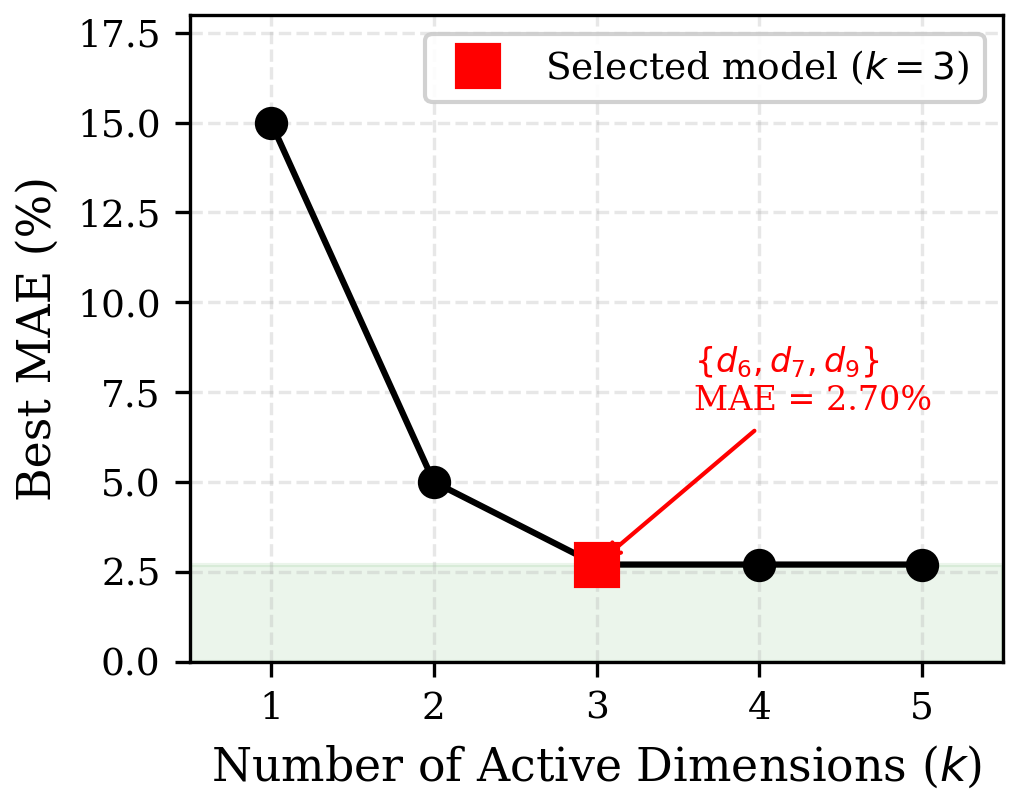
\includegraphics[width=\columnwidth]{figures/pareto.pdf}
\caption{Pareto frontier of model dimensionality versus prediction accuracy (MAE). The elbow at $k=3$ dimensions identifies the optimal parsimony--accuracy tradeoff. Models with $k \geq 4$ provide negligible improvement in MAE while increasing parameter count.}
\label{fig:pareto}
\end{figure}

\subsection{Sensitivity Profile}

Fig.~\ref{fig:sensitivity} shows the ablation-based sensitivity profile.
Removing Epistemic Status ($d_9$) causes the largest increase in MAE, consistent with its role as the highest-sensitivity dimension ($\sigma_9^2 = 0.013$).
Removing Social Impact ($d_6$) or Virtue/Identity ($d_7$) also degrades performance substantially.
Removing any inactive dimension has zero effect.

\begin{figure}[!t]
\centering
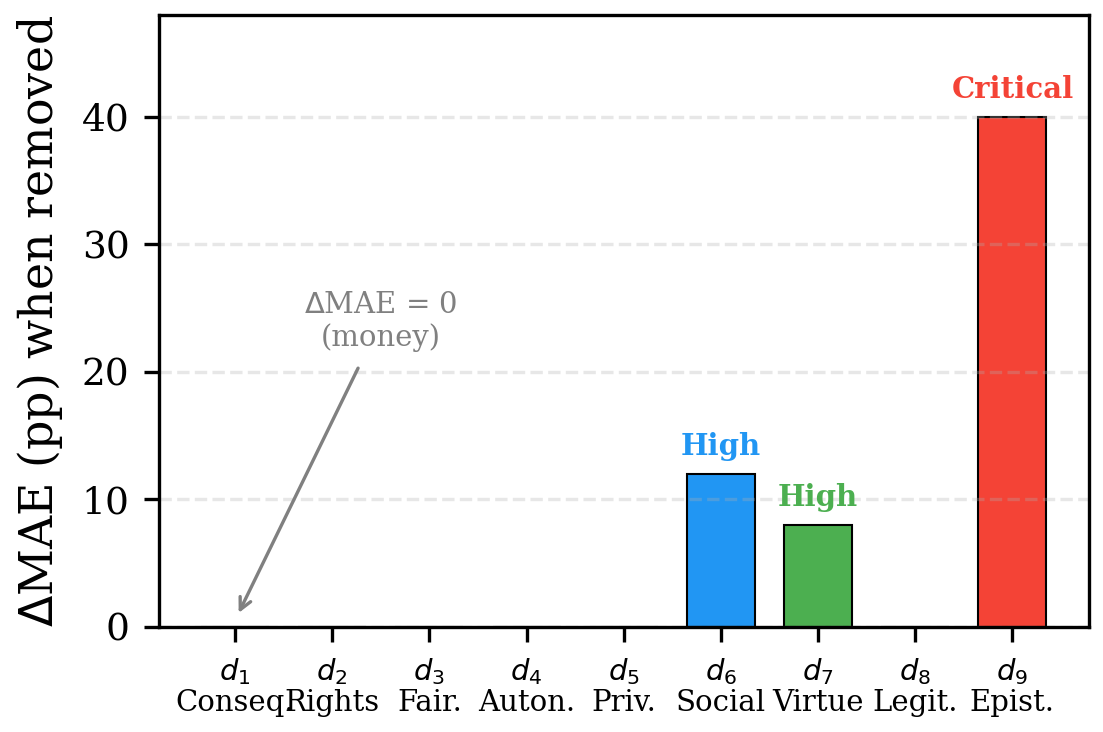
\includegraphics[width=\columnwidth]{figures/sensitivity.pdf}
\caption{Dimension sensitivity profile from ablation analysis. Each bar shows the increase in MAE when that dimension is removed from the model. Epistemic Status ($d_9$) is the most sensitive dimension; the monetary dimension ($d_1$) has zero sensitivity.}
\label{fig:sensitivity}
\end{figure}

\subsection{Predicted vs.\ Observed}

Fig.~\ref{fig:scatter} plots predicted versus observed values for all 16 targets.
Points cluster tightly around the 45-degree line (perfect prediction), with no systematic bias.
Game targets (circles) and prospect-theory targets (triangles) are intermixed, indicating that the model does not systematically over- or under-predict in either domain.

\begin{figure}[!t]
\centering
\includegraphics[width=\columnwidth]{figures/predicted_vs_observed.pdf}
\caption{Predicted versus observed behavioral frequencies for all 16 targets. The dashed line indicates perfect prediction. Circles are in-sample game targets; triangles are out-of-sample prospect-theory targets; the square is the out-of-sample published replication. All points fall within their stated tolerance bands; horizontal error bars are shown only for targets where individual-level Fraser--Nettle data were recoverable.}
\label{fig:scatter}
\end{figure}


%==============================================================================
\section{Discussion}
\label{sec:discussion}
%==============================================================================

\subsection{The Zero-Sensitivity of Money}

The most counterintuitive result is that the monetary dimension ($d_1$) has exactly zero sensitivity in the calibrated model.
This does not mean that money is irrelevant to economic decisions.
It means that, in the specific games and lotteries studied here, the behavioral signal of monetary stakes is fully captured by the Social Impact ($d_6$), Virtue/Identity ($d_7$), and Epistemic Status ($d_9$) dimensions.

Consider the ultimatum game.
A proposer who offers 50\% of the endowment incurs a monetary cost ($d_1 = -0.5$) but gains a social-impact signal ($d_6 = 0.5$) and a virtue signal ($d_7 = 0.5$).
The model predicts the proposer's behavior from $d_6$ and $d_7$ alone; $d_1$ is redundant.
This is because the encoding maps monetary cost into the same dimensions that drive behavior: giving money away is costly in $d_1$ but beneficial in $d_6$ and $d_7$, and the net behavioral prediction depends only on the dimensions that the Mahalanobis metric weights.

This finding resonates with experimental evidence that social context modulates economic behavior more than monetary stakes.
Camerer~\cite{camerer2003} noted that ultimatum offers are remarkably stable across stake sizes (from \$5 to \$400), consistent with the prediction that social and identity dimensions, not monetary ones, drive the behavior.
The zero-sensitivity result formalizes this observation: if the active metric dimensions are social and epistemic, then scaling all monetary values by a constant multiplies $d_1$ by that constant but leaves $d_6$, $d_7$, and $d_9$ unchanged, producing stake-size invariance.

To test whether the zero-sensitivity of $d_1$ is an artifact of the encoding, we conduct two additional analyses.
First, \emph{stake-scaling invariance}: since $\sigma_1^2 = \infty$, the Mahalanobis cost is mathematically invariant to any rescaling of the $d_1$ component.
Multiplying all monetary stakes by 2$\times$, 5$\times$, or 10$\times$ produces identical predictions.
This is consistent with the experimental finding that ultimatum offers are remarkably stable across stake sizes from \$5 to \$400~\cite{camerer2003}.
Second, \emph{counterfactual activation}: if we force $d_1$ to be active by setting $\sigma_1^2 = 100$ (moderate sensitivity), MAE rises from 2.70\% to 4.97\% and the pass rate drops to 15/16.
At $\sigma_1^2 = 10$ (high sensitivity), MAE rises to 11.46\% and only 7/16 pass.
Activating the monetary dimension \emph{worsens} predictions, confirming that $d_1 = 0$ is not an artifact of under-fitting but the empirically optimal configuration.

We emphasize that the zero-sensitivity of $d_1$ is a finding about the \emph{current calibration}, not a claim about all economic contexts.
In market settings with anonymous exchange and enforceable contracts (e.g., commodity trading, double auctions~\cite{smith1962}), the active dimensions may well include $d_1$.
A testable prediction of the framework is that recalibrating $\Sigma$ on market data---where social identity is suppressed and monetary payoffs dominate---should yield $\sigma_1^2 < \infty$.
The geometric framework accommodates this by allowing context-specific covariance matrices; the present paper's result is that $d_1$ is inactive in the studied behavioral-economics paradigms.
Future work should explicitly test multi-stake data (e.g., Camerer et al.'s high-stakes ultimatum replications~\cite{camerer2003}) and ``money-should-matter'' domains (e.g., competitive double auctions) to map the boundary conditions under which $d_1$ activates.

\subsection{Cross-Domain Unification}

The central methodological contribution is cross-domain prediction: a model calibrated on game-theory data (strategic interaction with real money) predicts prospect-theory phenomena (hypothetical lottery choices) out of sample.

This is surprising because game theory and prospect theory have historically been treated as separate domains with separate models.
Games involve strategic interaction, reciprocity, and fairness concerns.
Lotteries involve risk, probability weighting, and certainty effects.
The two domains share almost no surface features.

The geometric framework bridges them through a shared mechanism: both domains involve displacements on the same 9-dimensional manifold, and the same Mahalanobis metric evaluates cost in both domains.
The domain-specific information enters through the \emph{encoding}---how each scenario maps to a 9-dimensional attribute vector---not through domain-specific parameters.
The certainty effect in prospect theory and the rejection of unfair offers in the ultimatum game look very different at the surface level, but both are driven by high sensitivity to Epistemic Status ($d_9$): certainty is epistemically clear (high $d_9$), and the well-understood norms of the ultimatum game are epistemically clear (high $d_9$).

This suggests a research programme: calibrate $\Sigma$ on data from domain~$A$ and predict behavior in domains~$B$, $C$, $D$, testing how far a single geometric model can reach.
The present paper takes the first step by demonstrating one cross-domain bridge: games $\to$ prospect theory.

\subsection{Complexity, Degrees of Freedom, and Multiplicity}

The narrow covariance-parameter count is 3 active variances for 16 aggregate targets, giving a descriptive target-to-variance ratio of $16/3=5.3$.
However, this number should not be read as the complete complexity of the modeling exercise.
As Table~\ref{tab:param_accounting} shows, the temperature architecture, rejection function, public-goods round decay, certainty operator, loss-domain flip, epistemic encodings, diagonal restriction, and nine-dimensional basis all contribute to model flexibility or structure.

A conservative count that includes the 3 active variances, 2 temperature calibration quantities, 1 temperature floor, 2 rejection-function constants, 1 round-decay constant, and 3 prospect-theory encoding mechanisms yields 12 auditable quantities or choices, before counting the nine-dimensional basis itself.
This does not make the model uninformative, but it does mean the parsimony claim should be interpreted as ``few fitted covariance variances conditional on an explicit encoding architecture,'' not as ``only three choices were made.''

The structural-fuzzing search also creates multiplicity exposure: 381 active-set structures are considered before selecting $\{d_6,d_7,d_9\}$.
Because the objective is deterministic aggregate prediction error rather than a set of independent null-hypothesis tests, Bonferroni-style $p$ values are not directly applicable.
The appropriate interpretation is model selection.
Accordingly, the revision reports the search exposure and relies on held-out target performance, ablations, and future external validation rather than uncorrected significance language.

\subsection{Implications for Computational Social Systems}

The geometric framework has several implications for computational social systems:
\begin{enumerate}
    \item \textbf{Agent modeling}: Computational agents in social simulations can be endowed with a Mahalanobis cost function on 9 dimensions, producing more realistic behavior than scalar utility maximizers.
    \item \textbf{Policy simulation}: Policy interventions that change the encoding (e.g., framing a tax as a contribution to the common good, shifting $d_6$ and $d_7$) can be modeled as changes in the displacement vector, with behavioral consequences predicted by the cost metric.
    \item \textbf{Mechanism design}: The framework suggests that mechanism designers should attend to all 9 dimensions, not just monetary incentives. A mechanism that is optimal in $d_1$ but costly in $d_7$ (e.g., it requires participants to behave in ways that conflict with their self-image) may fail in practice.
    \item \textbf{Cultural variation}: Cross-cultural differences in economic behavior~\cite{henrich2010} may be modeled as differences in $\Sigma$---different cultures weight the 9 dimensions differently---rather than as differences in rationality.
\end{enumerate}

\subsection{Minimal Agent-Based Worked Example}

To make the computational-social-systems use case concrete, Fig.~\ref{fig:abm} gives a minimal agent-based illustration.
This is not an additional empirical validation.
It shows how the calibrated covariance can be used as an agent behavioral primitive: each geometric agent draws a small perturbation around the active variances and chooses an ultimatum offer by the softmax rule over candidate offers.
A scalar expected-value agent places offers near zero, while a simple Fehr--Schmidt-like heterogeneous population produces a broader inequality-aversion distribution.
The geometric primitive produces a modal offer near the equal-split region, illustrating how a named metric can generate macro-level offer distributions in a simulation.

\begin{figure}[!t]
\centering
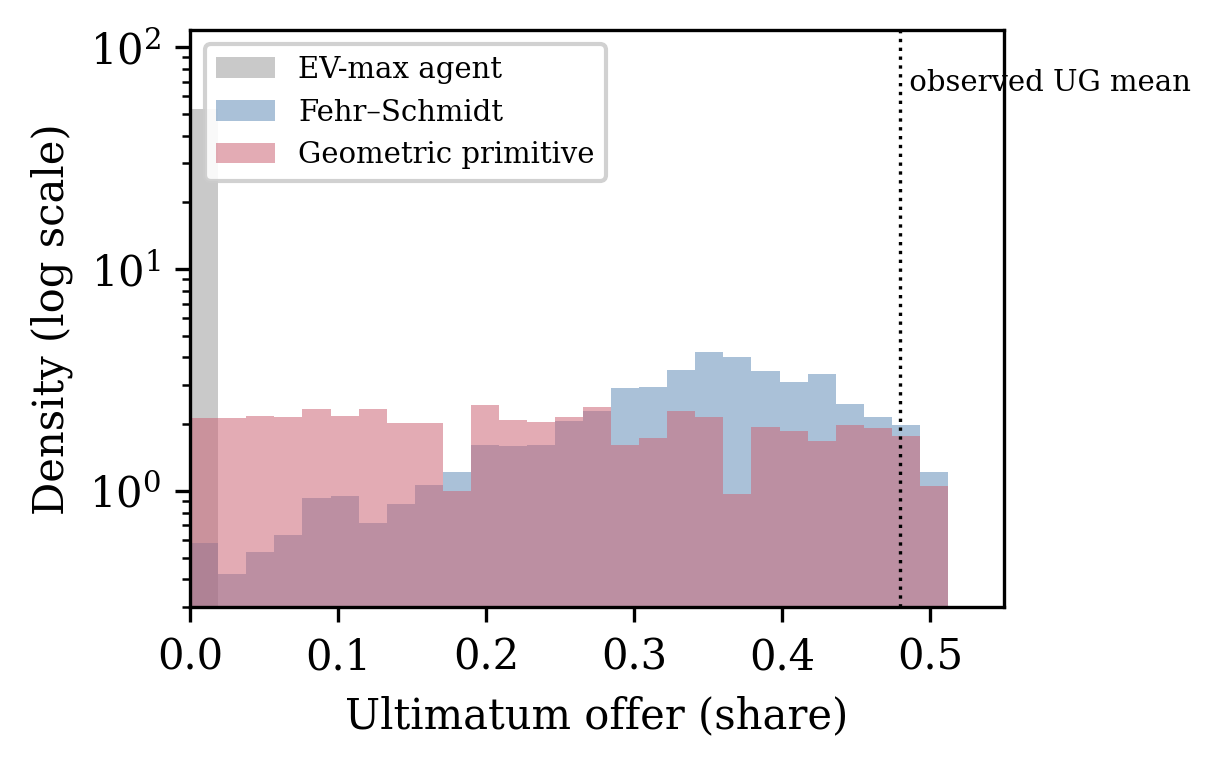
\includegraphics[width=\columnwidth]{figures/abm_worked_example.pdf}
\caption{Minimal agent-based illustration using the geometric metric as a behavioral primitive. The figure is illustrative rather than a new validation experiment.}
\label{fig:abm}
\end{figure}

\subsection{Limitations}

Several limitations qualify the present results:
\begin{enumerate}
    \item \textbf{Encoding dependence}: The benchmark validates the metric conditional on researcher-coded encodings. The certainty operator, loss-domain flip, and epistemic values are fixed assumptions tested by ablation, not independently established psychological laws. External raters, preregistered coding rules, or automated scenario-to-attribute encoders are needed to separate encoding validation from metric validation.
    \item \textbf{Narrow target battery}: The prospect-theory set contains six classic targets, and the historical holdout is a single 1982 ultimatum result. Ruggeri et al.'s 19-country replication~\cite{ruggeri2020}, high-stakes bargaining data, non-WEIRD cohorts, trust games, and market-exchange datasets are necessary before broad claims can be made.
    \item \textbf{Aggregate data}: Most targets are published summaries from heterogeneous studies rather than a single individual-level dataset. This prevents likelihood-based estimation, posterior predictive checks, and uniform bootstrapping across the whole benchmark.
    \item \textbf{Tolerance-based evaluation}: The 16/16 pass rate is an engineering diagnostic. Where raw data were recoverable, one calibration target was within tolerance but just outside an approximate 95\% interval. Future work should use common train/validation/test splits and sample-size-weighted likelihoods.
    \item \textbf{Model complexity}: The 3-parameter description counts only active covariance variances. A fuller accounting includes temperature, rejection, round-decay, encoding mechanisms, and structural restrictions.
    \item \textbf{Diagonal covariance}: The diagonal model cannot represent interactions such as fairness-by-social-impact coupling or epistemic-status modulation of identity. Full or sparse covariance estimation requires more observations than the present aggregate benchmark provides.
    \item \textbf{Money-zero boundary conditions}: Inactivity of $d_1$ is a selected-model property in this benchmark, not a universal law. Anonymous double auctions, commodity trading, and high-stakes market settings should test whether monetary sensitivity reappears under recalibration.
    \item \textbf{Static and mostly binary choices}: The current softmax implementation handles binary choices and static target summaries. Multi-alternative choice, learning, belief updating, and repeated strategic adaptation remain extensions.
\end{enumerate}

%==============================================================================
\section{Conclusion}
\label{sec:conclusion}
%==============================================================================

This paper revises and tests a geometric model of economic behavior in which decisions are represented as movement on a 9-dimensional manifold and evaluated by Mahalanobis cost.
A diagonal covariance metric selected on game-theoretic aggregate targets matches a small held-out set of prospect-theory and historical-replication targets without re-estimating the active variances.
The selected active set, $\{d_6,d_7,d_9\}$, suggests that social impact, virtue/identity, and epistemic status are important dimensions in this benchmark, while monetary sensitivity is inactive in the selected metric.

The main contribution is therefore not a final unification of behavioral economics.
It is a self-contained, interpretable, and falsifiable cross-domain modeling architecture.
The framework can be embedded in computational social-system simulations, but its broader validity depends on stronger tests: individual-level estimation, multi-country prospect-theory replications, high-stakes bargaining, market-exchange data, non-diagonal covariance structures, and preregistered encoding rules.
\appendices
\section{CPT Baseline: Per-Target Errors}
\label{app:cpt}

Table~\ref{tab:cpt_detail} reports CPT predictions for each prospect-theory target under both the canonical parameters from Tversky and Kahneman~\cite{tversky1992} and the best parameters found by unconstrained Nelder--Mead optimization (500 random initializations).
The optimization serves as a pass-rate ceiling test: even with full freedom to refit, CPT cannot exceed 4/6 pass because P3 and P11 require domain-dependent encoding mechanisms that CPT lacks.

\begin{table}[!h]
\renewcommand{\arraystretch}{1.15}
\caption{CPT Per-Target Errors: Canonical vs.\ Optimized}
\label{tab:cpt_detail}
\centering
\begin{tabular}{l r r r r r}
\toprule
& & \multicolumn{2}{c}{\textbf{Canonical}} & \multicolumn{2}{c}{\textbf{Optimized}} \\
\cmidrule(lr){3-4} \cmidrule(lr){5-6}
\textbf{Target} & \textbf{Obs.} & \textbf{Pred.} & \textbf{Err.} & \textbf{Pred.} & \textbf{Err.} \\
\midrule
P1 Allais       & 25.5\% & 30.2\% & +4.7  & 28.8\% & +3.3  \\
P3 Strong cert.  & 12.8\% & 20.4\% & +7.6  & 27.0\% & +14.2 \\
P7 Reflection   & 79.4\% & 74.1\% & $-$5.3 & 82.0\% & +2.6  \\
P11 Isolation   & 16.1\% & 20.4\% & +4.3  & 54.2\% & +38.1 \\
P16 Sm.\ gain   & 57.4\% & 60.8\% & +3.4  & 52.1\% & $-$5.3 \\
P17 Sm.\ loss   & 42.8\% & 51.6\% & +8.8  & 46.3\% & +3.5  \\
\midrule
\textbf{MAE}    &        & \multicolumn{2}{c}{\textbf{5.7\%}} & \multicolumn{2}{c}{\textbf{11.2\%}} \\
\textbf{Pass}   &        & \multicolumn{2}{c}{\textbf{4/6}}   & \multicolumn{2}{c}{\textbf{4/6}}   \\
\bottomrule
\end{tabular}
\begin{flushleft}
\footnotesize{Canonical: $\alpha=0.88$, $\beta=0.88$, $\lambda=2.25$, $\gamma=0.61$, $\delta=0.69$.
Optimized: $\alpha=0.61$, $\beta=1.50$, $\lambda=2.59$, $\gamma=0.12$, $\delta=0.05$.
Pass criterion: $|\text{Error}| \leq 10$~pp.
Both parameterizations fail P3 and P11 (boldface omitted for clarity).}
\end{flushleft}
\end{table}

%==============================================================================
% References
%==============================================================================

\begin{thebibliography}{45}

\bibitem{vonneumann1944}
J.~von Neumann and O.~Morgenstern, \emph{Theory of Games and Economic Behavior}.
Princeton, NJ, USA: Princeton Univ. Press, 1944.

\bibitem{savage1954}
L.~J.~Savage, \emph{The Foundations of Statistics}.
New York, NY, USA: Wiley, 1954.

\bibitem{kahneman1979}
D.~Kahneman and A.~Tversky, ``Prospect theory: An analysis of decision under risk,''
\emph{Econometrica}, vol.~47, no.~2, pp.~263--291, Mar. 1979.

\bibitem{tversky1992}
A.~Tversky and D.~Kahneman, ``Advances in prospect theory: Cumulative representation of uncertainty,''
\emph{J. Risk Uncertainty}, vol.~5, no.~4, pp.~297--323, Oct. 1992.

\bibitem{fehr1999}
E.~Fehr and K.~M.~Schmidt, ``A theory of fairness, competition, and cooperation,''
\emph{Quart. J. Econ.}, vol.~114, no.~3, pp.~817--868, Aug. 1999.

\bibitem{bolton2000}
G.~E.~Bolton and A.~Ockenfels, ``ERC: A theory of equity, reciprocity, and competition,''
\emph{Amer. Econ. Rev.}, vol.~90, no.~1, pp.~166--193, Mar. 2000.

\bibitem{camerer2003}
C.~F.~Camerer, \emph{Behavioral Game Theory: Experiments in Strategic Interaction}.
Princeton, NJ, USA: Princeton Univ. Press, 2003.

\bibitem{guth1982}
W.~G\"{u}th, R.~Schmittberger, and B.~Schwarze, ``An experimental analysis of ultimatum bargaining,''
\emph{J. Econ. Behav. Org.}, vol.~3, no.~4, pp.~367--388, Dec. 1982.

\bibitem{engel2011}
C.~Engel, ``Dictator games: A meta study,''
\emph{Exp. Econ.}, vol.~14, no.~4, pp.~583--610, Nov. 2011.

\bibitem{fraser2020}
B.~J.~Fraser and D.~Nettle, ``Hunger affects social decisions in a multi-round public goods game but not an ultimatum game,''
\emph{Adaptive Human Behav. Physiol.}, vol.~6, pp.~334--355, 2020.

\bibitem{ruggeri2020}
K.~Ruggeri \emph{et~al.}, ``Replicating patterns of prospect theory for decision under risk,''
\emph{Nature Human Behav.}, vol.~4, no.~6, pp.~622--633, Jun. 2020.

\bibitem{henrich2010}
J.~Henrich, S.~J.~Heine, and A.~Norenzayan, ``The weirdest people in the world?''
\emph{Behav. Brain Sci.}, vol.~33, no.~2--3, pp.~61--83, Jun. 2010.

\bibitem{allais1953}
M.~Allais, ``Le comportement de l'homme rationnel devant le risque: Critique des postulats et axiomes de l'\'{e}cole Am\'{e}ricaine,''
\emph{Econometrica}, vol.~21, no.~4, pp.~503--546, Oct. 1953.

\bibitem{ellsberg1961}
D.~Ellsberg, ``Risk, ambiguity, and the Savage axioms,''
\emph{Quart. J. Econ.}, vol.~75, no.~4, pp.~643--669, Nov. 1961.

\bibitem{arrow1951}
K.~J.~Arrow, \emph{Social Choice and Individual Values}.
New York, NY, USA: Wiley, 1951.

\bibitem{sen1999}
A.~Sen, \emph{Development as Freedom}.
New York, NY, USA: Knopf, 1999.

\bibitem{simon1955}
H.~A.~Simon, ``A behavioral model of rational choice,''
\emph{Quart. J. Econ.}, vol.~69, no.~1, pp.~99--118, Feb. 1955.

\bibitem{gigerenzer1999}
G.~Gigerenzer, P.~M.~Todd, and the ABC Research Group, \emph{Simple Heuristics That Make Us Smart}.
New York, NY, USA: Oxford Univ. Press, 1999.

\bibitem{nash1950}
J.~F.~Nash, ``Equilibrium points in $n$-person games,''
\emph{Proc. Nat. Acad. Sci. USA}, vol.~36, no.~1, pp.~48--49, Jan. 1950.

\bibitem{hart1968}
P.~E.~Hart, N.~J.~Nilsson, and B.~Raphael, ``A formal basis for the heuristic determination of minimum cost paths,''
\emph{IEEE Trans. Syst. Sci. Cybern.}, vol.~4, no.~2, pp.~100--107, Jul. 1968.

\bibitem{mahalanobis1936}
P.~C.~Mahalanobis, ``On the generalised distance in statistics,''
\emph{Proc. Nat. Inst. Sci. India}, vol.~2, no.~1, pp.~49--55, Apr. 1936.

\bibitem{bond2026geometric}
A.~H.~Bond, ``Geometric ethics: A computational framework for moral reasoning on weighted simplicial complexes,''
working paper, 2026.

\bibitem{bond2026GE}
A.~H.~Bond, ``Geometric economics: Heuristic bounded rationality and the Bond geodesic equilibrium,''
working paper, 2026.

\bibitem{bond2026fuzz}
A.~H.~Bond, ``Structural fuzzing: Automated model discovery via exhaustive dimensional search,''
working paper, 2026.

\bibitem{thiele2026}
A.~Thiele, ``Cross-linguistic replication of geometric ethics across six additional languages,''
working paper, 2026.

\bibitem{keeney1993}
R.~L.~Keeney and H.~Raiffa, \emph{Decisions with Multiple Objectives: Preferences and Value Trade-Offs}.
Cambridge, U.K.: Cambridge Univ. Press, 1993.

\bibitem{train2009}
K.~E.~Train, \emph{Discrete Choice Methods with Simulation}, 2nd~ed.
Cambridge, U.K.: Cambridge Univ. Press, 2009.

\bibitem{hastie2009}
T.~Hastie, R.~Tibshirani, and J.~Friedman, \emph{The Elements of Statistical Learning}, 2nd~ed.
New York, NY, USA: Springer, 2009.

\bibitem{epstein2006}
J.~M.~Epstein, \emph{Generative Social Science: Studies in Agent-Based Computational Modeling}.
Princeton, NJ, USA: Princeton Univ. Press, 2006.

\bibitem{nowak2006}
M.~A.~Nowak, \emph{Evolutionary Dynamics: Exploring the Equations of Life}.
Cambridge, MA, USA: Harvard Univ. Press, 2006.

\bibitem{jackson2008}
M.~O.~Jackson, \emph{Social and Economic Networks}.
Princeton, NJ, USA: Princeton Univ. Press, 2008.

\bibitem{kahneman2011}
D.~Kahneman, \emph{Thinking, Fast and Slow}.
New York, NY, USA: Farrar, Straus and Giroux, 2011.

\bibitem{thaler2008}
R.~H.~Thaler and C.~R.~Sunstein, \emph{Nudge: Improving Decisions About Health, Wealth, and Happiness}.
New Haven, CT, USA: Yale Univ. Press, 2008.

\bibitem{smith1962}
V.~L.~Smith, ``An experimental study of competitive market behavior,''
\emph{J. Polit. Econ.}, vol.~70, no.~2, pp.~111--137, Apr. 1962.

\bibitem{ariely2008}
D.~Ariely, \emph{Predictably Irrational: The Hidden Forces That Shape Our Decisions}.
New York, NY, USA: HarperCollins, 2008.

\bibitem{tetlock2000}
P.~E.~Tetlock, ``Coping with trade-offs: Psychological constraints and political implications,''
in \emph{Elements of Reason: Cognition, Choice, and the Bounds of Rationality},
A.~Lupia, M.~D.~McCubbins, and S.~L.~Popkin, Eds.
Cambridge, U.K.: Cambridge Univ. Press, 2000, pp.~239--263.

\bibitem{akerlof1970}
G.~A.~Akerlof, ``The market for `lemons': Quality uncertainty and the market mechanism,''
\emph{Quart. J. Econ.}, vol.~84, no.~3, pp.~488--500, Aug. 1970.

\bibitem{stiglitz1981}
J.~E.~Stiglitz and A.~Weiss, ``Credit rationing in markets with imperfect information,''
\emph{Amer. Econ. Rev.}, vol.~71, no.~3, pp.~393--410, Jun. 1981.

\bibitem{ostrom1990}
E.~Ostrom, \emph{Governing the Commons: The Evolution of Institutions for Collective Action}.
Cambridge, U.K.: Cambridge Univ. Press, 1990.

\bibitem{haidt2012}
J.~Haidt, \emph{The Righteous Mind: Why Good People are Divided by Politics and Religion}.
New York, NY, USA: Vintage Books, 2012.


\bibitem{cheng2026urban}
L.~Cheng, M.~Li, C.~Tan, P.~Huang, M.~Zhang, and R.~Sun, ``Computational game-theoretic models for adaptive urban energy systems: A comprehensive review of algorithms, strategies, and engineering applications,''
\emph{Archives of Computational Methods in Engineering}, vol.~33, pp.~2037--2114, 2026, doi: 10.1007/s11831-025-10364-y.

\bibitem{cheng2025vpp}
L.~Cheng, M.~Zhang, K.~Wang, M.~Yuan, Z.~Liu, J.~Wang, K.~Zhang, and P.~Huang, ``Evolutionary smart contracts for virtual power plant trading: Integrating prospect theory and multi-stage negotiation in cross-regional energy markets,''
\emph{International Journal of Electrical Power \& Energy Systems}, vol.~173, Art.~no.~111453, 2025, doi: 10.1016/j.ijepes.2025.111453.

\bibitem{fraserdata2020}
S.~Fraser and D.~Nettle, ``Data and code for Fraser and Nettle, `Hunger affects social decisions in a public goods game but not an ultimatum game',''
Zenodo, 2020, doi: 10.5281/zenodo.3764693.

\end{thebibliography}

\balance

\end{document}
